\documentclass{standalone}
\usepackage{tikz}
\usetikzlibrary{patterns, positioning}

\begin{document}
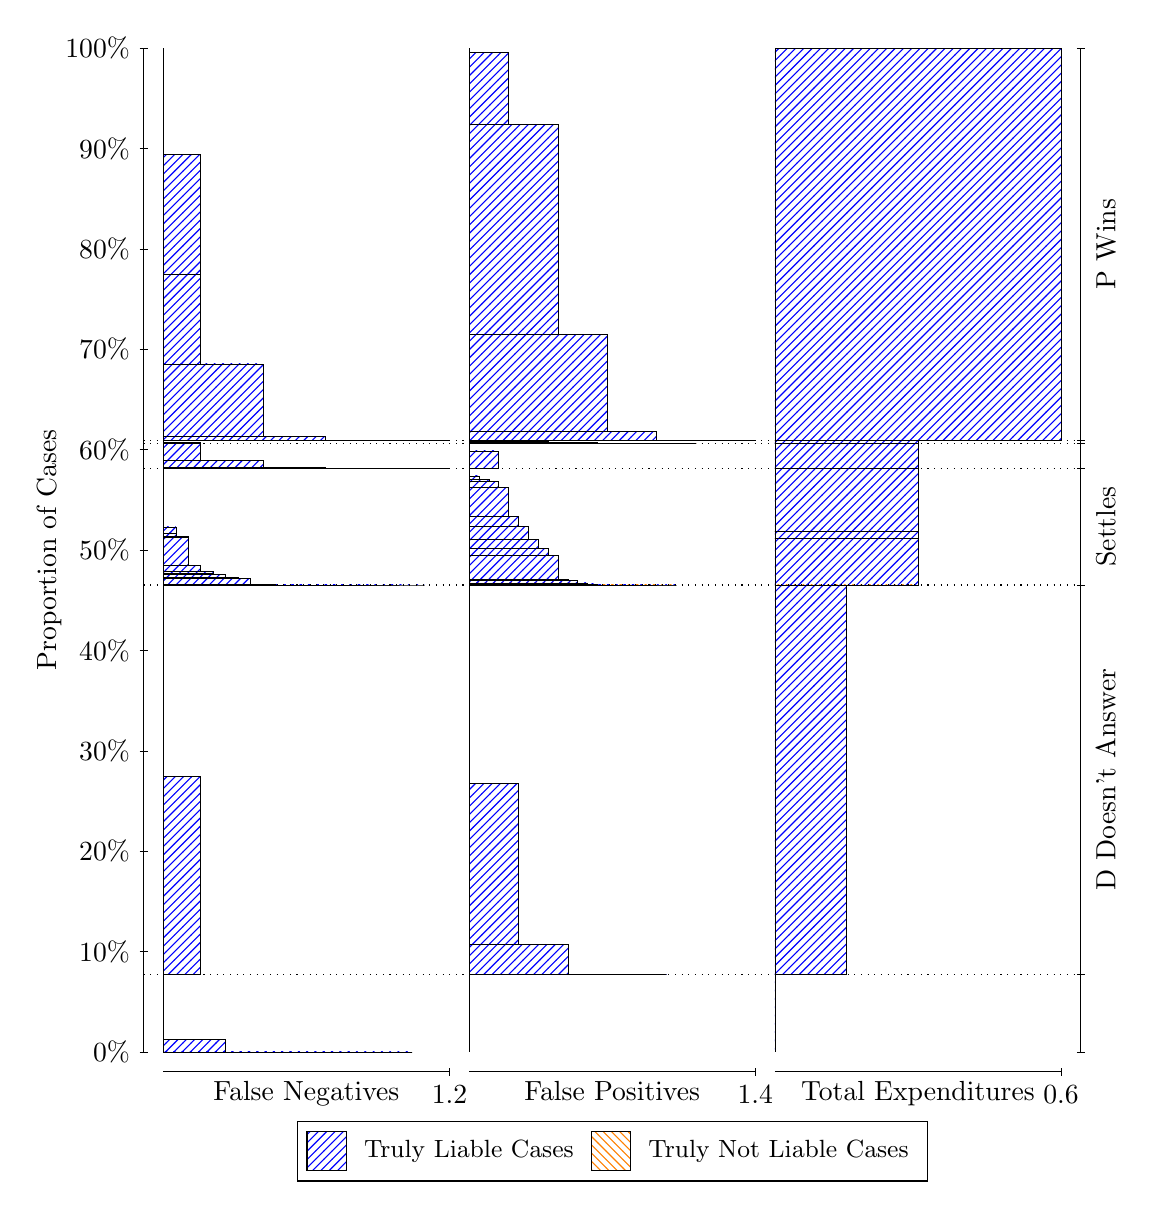
\begin{tikzpicture}
\draw[black, very thin] (1.5,1.75) -- (1.5,14.5);
\node[rotate=90, anchor=center] at (0.3, 8.125) {Proportion of Cases};
\draw[black, very thin] (1.45,1.75) -- (1.55,1.75);
\node[anchor=east] at (1.45, 1.75) {0\%};
\draw[black, very thin] (1.45,3.025) -- (1.55,3.025);
\node[anchor=east] at (1.45, 3.025) {10\%};
\draw[black, very thin] (1.45,4.3) -- (1.55,4.3);
\node[anchor=east] at (1.45, 4.3) {20\%};
\draw[black, very thin] (1.45,5.575) -- (1.55,5.575);
\node[anchor=east] at (1.45, 5.575) {30\%};
\draw[black, very thin] (1.45,6.85) -- (1.55,6.85);
\node[anchor=east] at (1.45, 6.85) {40\%};
\draw[black, very thin] (1.45,8.125) -- (1.55,8.125);
\node[anchor=east] at (1.45, 8.125) {50\%};
\draw[black, very thin] (1.45,9.4) -- (1.55,9.4);
\node[anchor=east] at (1.45, 9.4) {60\%};
\draw[black, very thin] (1.45,10.675) -- (1.55,10.675);
\node[anchor=east] at (1.45, 10.675) {70\%};
\draw[black, very thin] (1.45,11.95) -- (1.55,11.95);
\node[anchor=east] at (1.45, 11.95) {80\%};
\draw[black, very thin] (1.45,13.225) -- (1.55,13.225);
\node[anchor=east] at (1.45, 13.225) {90\%};
\draw[black, very thin] (1.45,14.5) -- (1.55,14.5);
\node[anchor=east] at (1.45, 14.5) {100\%};

\draw[black, very thin] (13.4,1.75) -- (13.4,14.5);
\draw[black, very thin] (13.35,1.75) -- (13.45,1.75);
\node[anchor=west] at (13.35, 1.75) {};
\draw[black, very thin] (13.35,2.7357) -- (13.45,2.7357);
\node[anchor=west] at (13.35, 2.7357) {};
\draw[black, very thin] (13.35,7.6806) -- (13.45,7.6806);
\node[anchor=west] at (13.35, 7.6806) {};
\draw[black, very thin] (13.35,9.1652) -- (13.45,9.1652);
\node[anchor=west] at (13.35, 9.1652) {};
\draw[black, very thin] (13.35,9.4822) -- (13.45,9.4822);
\node[anchor=west] at (13.35, 9.4822) {};
\draw[black, very thin] (13.35,9.5191) -- (13.45,9.5191);
\node[anchor=west] at (13.35, 9.5191) {};
\draw[black, very thin] (13.35,14.5) -- (13.45,14.5);
\node[anchor=west] at (13.35, 14.5) {};

\draw[black, very thin, pattern color=blue, pattern=north east lines] (1.75,1.75) rectangle (4.9094,1.75);
\draw[black, very thin, pattern color=blue, pattern=north east lines] (1.75,1.75) rectangle (4.1196,1.75);
\draw[black, very thin, pattern color=blue, pattern=north east lines] (1.75,1.75) rectangle (3.3297,1.7514);
\draw[black, very thin, pattern color=blue, pattern=north east lines] (1.75,1.7514) rectangle (2.5399,1.9114);
\draw[black, very thin, pattern color=orange, pattern=north west lines] (1.75,1.9114) rectangle (1.75,1.9114);
\draw[black, very thin, pattern color=blue, pattern=north east lines] (1.75,1.9114) rectangle (1.75,2.7357);
\draw[black, very thin, pattern color=blue, pattern=north east lines] (1.75,2.7357) rectangle (2.2239,5.2537);
\draw[black, very thin, pattern color=orange, pattern=north west lines] (1.75,5.2537) rectangle (1.75,5.2537);
\draw[black, very thin, pattern color=blue, pattern=north east lines] (1.75,5.2537) rectangle (1.75,7.6806);
\draw[black, very thin, pattern color=blue, pattern=north east lines] (1.75,7.6806) rectangle (5.0674,7.6806);
\draw[black, very thin, pattern color=blue, pattern=north east lines] (1.75,7.6806) rectangle (4.7514,7.6806);
\draw[black, very thin, pattern color=blue, pattern=north east lines] (1.75,7.6806) rectangle (4.4355,7.6806);
\draw[black, very thin, pattern color=blue, pattern=north east lines] (1.75,7.6806) rectangle (4.2775,7.6806);
\draw[black, very thin, pattern color=blue, pattern=north east lines] (1.75,7.6806) rectangle (4.1196,7.6806);
\draw[black, very thin, pattern color=blue, pattern=north east lines] (1.75,7.6806) rectangle (3.9616,7.6806);
\draw[black, very thin, pattern color=blue, pattern=north east lines] (1.75,7.6806) rectangle (3.8036,7.6807);
\draw[black, very thin, pattern color=blue, pattern=north east lines] (1.75,7.6807) rectangle (3.6457,7.6808);
\draw[black, very thin, pattern color=blue, pattern=north east lines] (1.75,7.6808) rectangle (3.4877,7.6815);
\draw[black, very thin, pattern color=blue, pattern=north east lines] (1.75,7.6815) rectangle (3.3297,7.6816);
\draw[black, very thin, pattern color=blue, pattern=north east lines] (1.75,7.6816) rectangle (3.1717,7.6822);
\draw[black, very thin, pattern color=blue, pattern=north east lines] (1.75,7.6822) rectangle (3.1717,7.6839);
\draw[black, very thin, pattern color=blue, pattern=north east lines] (1.75,7.6839) rectangle (3.0138,7.6869);
\draw[black, very thin, pattern color=blue, pattern=north east lines] (1.75,7.6869) rectangle (2.8558,7.7606);
\draw[black, very thin, pattern color=blue, pattern=north east lines] (1.75,7.7606) rectangle (2.6978,7.7634);
\draw[black, very thin, pattern color=blue, pattern=north east lines] (1.75,7.7634) rectangle (2.6978,7.7798);
\draw[black, very thin, pattern color=blue, pattern=north east lines] (1.75,7.7798) rectangle (2.5399,7.8195);
\draw[black, very thin, pattern color=blue, pattern=north east lines] (1.75,7.8195) rectangle (2.3819,7.8326);
\draw[black, very thin, pattern color=blue, pattern=north east lines] (1.75,7.8326) rectangle (2.3819,7.8495);
\draw[black, very thin, pattern color=blue, pattern=north east lines] (1.75,7.8495) rectangle (2.2239,7.9293);
\draw[black, very thin, pattern color=blue, pattern=north east lines] (1.75,7.9293) rectangle (2.0659,8.2881);
\draw[black, very thin, pattern color=blue, pattern=north east lines] (1.75,8.2881) rectangle (2.0659,8.2956);
\draw[black, very thin, pattern color=blue, pattern=north east lines] (1.75,8.2956) rectangle (1.908,8.3421);
\draw[black, very thin, pattern color=blue, pattern=north east lines] (1.75,8.3421) rectangle (1.908,8.4179);
\draw[black, very thin, pattern color=blue, pattern=north east lines] (1.75,8.4179) rectangle (1.75,8.419);
\draw[black, very thin, pattern color=orange, pattern=north west lines] (1.75,8.419) rectangle (1.75,8.419);
\draw[black, very thin, pattern color=blue, pattern=north east lines] (1.75,8.419) rectangle (1.75,9.1652);
\draw[black, very thin, pattern color=blue, pattern=north east lines] (1.75,9.1652) rectangle (5.3833,9.1652);
\draw[black, very thin, pattern color=blue, pattern=north east lines] (1.75,9.1652) rectangle (4.5935,9.1652);
\draw[black, very thin, pattern color=blue, pattern=north east lines] (1.75,9.1652) rectangle (3.8036,9.1741);
\draw[black, very thin, pattern color=blue, pattern=north east lines] (1.75,9.1741) rectangle (3.0138,9.2632);
\draw[black, very thin, pattern color=blue, pattern=north east lines] (1.75,9.2632) rectangle (2.2239,9.4822);
\draw[black, very thin, pattern color=orange, pattern=north west lines] (1.75,9.4822) rectangle (1.75,9.4822);
\draw[black, very thin, pattern color=blue, pattern=north east lines] (1.75,9.4822) rectangle (2.2239,9.4892);
\draw[black, very thin, pattern color=orange, pattern=north west lines] (1.75,9.4892) rectangle (1.75,9.4892);
\draw[black, very thin, pattern color=blue, pattern=north east lines] (1.75,9.4892) rectangle (1.75,9.5191);
\draw[black, very thin, pattern color=blue, pattern=north east lines] (1.75,9.5191) rectangle (5.3833,9.5191);
\draw[black, very thin, pattern color=blue, pattern=north east lines] (1.75,9.5191) rectangle (4.5935,9.5193);
\draw[black, very thin, pattern color=blue, pattern=north east lines] (1.75,9.5193) rectangle (3.8036,9.5706);
\draw[black, very thin, pattern color=blue, pattern=north east lines] (1.75,9.5706) rectangle (3.0138,10.488);
\draw[black, very thin, pattern color=blue, pattern=north east lines] (1.75,10.488) rectangle (2.2239,11.626);
\draw[black, very thin, pattern color=blue, pattern=north east lines] (1.75,11.626) rectangle (2.2239,13.154);
\draw[black, very thin, pattern color=orange, pattern=north west lines] (1.75,13.154) rectangle (1.75,13.154);
\draw[black, very thin, pattern color=blue, pattern=north east lines] (1.75,13.154) rectangle (1.75,14.5);
\draw[black, very thin, pattern color=orange, pattern=north west lines] (5.6333,1.75) rectangle (5.6333,1.75);
\draw[black, very thin, pattern color=blue, pattern=north east lines] (5.6333,1.75) rectangle (5.6333,2.7357);
\draw[black, very thin, pattern color=orange, pattern=north west lines] (5.6333,2.7357) rectangle (8.1391,2.7357);
\draw[black, very thin, pattern color=blue, pattern=north east lines] (5.6333,2.7357) rectangle (8.1391,2.7357);
\draw[black, very thin, pattern color=blue, pattern=north east lines] (5.6333,2.7357) rectangle (7.5126,2.7388);
\draw[black, very thin, pattern color=blue, pattern=north east lines] (5.6333,2.7388) rectangle (6.8862,3.1197);
\draw[black, very thin, pattern color=blue, pattern=north east lines] (5.6333,3.1197) rectangle (6.2598,5.1626);
\draw[black, very thin, pattern color=blue, pattern=north east lines] (5.6333,5.1626) rectangle (5.6333,7.6806);
\draw[black, very thin, pattern color=orange, pattern=north west lines] (5.6333,7.6806) rectangle (8.2644,7.6806);
\draw[black, very thin, pattern color=blue, pattern=north east lines] (5.6333,7.6806) rectangle (8.2644,7.6806);
\draw[black, very thin, pattern color=orange, pattern=north west lines] (5.6333,7.6806) rectangle (8.0138,7.6806);
\draw[black, very thin, pattern color=blue, pattern=north east lines] (5.6333,7.6806) rectangle (8.0138,7.6806);
\draw[black, very thin, pattern color=orange, pattern=north west lines] (5.6333,7.6806) rectangle (7.7632,7.6806);
\draw[black, very thin, pattern color=blue, pattern=north east lines] (5.6333,7.6806) rectangle (7.7632,7.6806);
\draw[black, very thin, pattern color=blue, pattern=north east lines] (5.6333,7.6806) rectangle (7.6379,7.6807);
\draw[black, very thin, pattern color=orange, pattern=north west lines] (5.6333,7.6807) rectangle (7.5126,7.6807);
\draw[black, very thin, pattern color=blue, pattern=north east lines] (5.6333,7.6807) rectangle (7.5126,7.6808);
\draw[black, very thin, pattern color=blue, pattern=north east lines] (5.6333,7.6808) rectangle (7.3874,7.6808);
\draw[black, very thin, pattern color=orange, pattern=north west lines] (5.6333,7.6808) rectangle (7.2621,7.6808);
\draw[black, very thin, pattern color=blue, pattern=north east lines] (5.6333,7.6808) rectangle (7.2621,7.6942);
\draw[black, very thin, pattern color=blue, pattern=north east lines] (5.6333,7.6942) rectangle (7.1368,7.7072);
\draw[black, very thin, pattern color=orange, pattern=north west lines] (5.6333,7.7072) rectangle (7.0115,7.7072);
\draw[black, very thin, pattern color=blue, pattern=north east lines] (5.6333,7.7072) rectangle (7.0115,7.7404);
\draw[black, very thin, pattern color=orange, pattern=north west lines] (5.6333,7.7404) rectangle (7.0115,7.7404);
\draw[black, very thin, pattern color=blue, pattern=north east lines] (5.6333,7.7404) rectangle (7.0115,7.7405);
\draw[black, very thin, pattern color=blue, pattern=north east lines] (5.6333,7.7405) rectangle (6.8862,7.7528);
\draw[black, very thin, pattern color=blue, pattern=north east lines] (5.6333,7.7528) rectangle (6.7609,7.755);
\draw[black, very thin, pattern color=orange, pattern=north west lines] (5.6333,7.755) rectangle (6.7609,7.755);
\draw[black, very thin, pattern color=blue, pattern=north east lines] (5.6333,7.755) rectangle (6.7609,8.0571);
\draw[black, very thin, pattern color=blue, pattern=north east lines] (5.6333,8.0571) rectangle (6.6356,8.1492);
\draw[black, very thin, pattern color=orange, pattern=north west lines] (5.6333,8.1492) rectangle (6.5103,8.1492);
\draw[black, very thin, pattern color=blue, pattern=north east lines] (5.6333,8.1492) rectangle (6.5103,8.2555);
\draw[black, very thin, pattern color=blue, pattern=north east lines] (5.6333,8.2555) rectangle (6.3851,8.4268);
\draw[black, very thin, pattern color=blue, pattern=north east lines] (5.6333,8.4268) rectangle (6.3851,8.4278);
\draw[black, very thin, pattern color=orange, pattern=north west lines] (5.6333,8.4278) rectangle (6.2598,8.4278);
\draw[black, very thin, pattern color=blue, pattern=north east lines] (5.6333,8.4278) rectangle (6.2598,8.5501);
\draw[black, very thin, pattern color=blue, pattern=north east lines] (5.6333,8.5501) rectangle (6.1345,8.5576);
\draw[black, very thin, pattern color=blue, pattern=north east lines] (5.6333,8.5576) rectangle (6.1345,8.9165);
\draw[black, very thin, pattern color=blue, pattern=north east lines] (5.6333,8.9165) rectangle (6.0092,8.9963);
\draw[black, very thin, pattern color=blue, pattern=north east lines] (5.6333,8.9963) rectangle (5.8839,9.0263);
\draw[black, very thin, pattern color=blue, pattern=north east lines] (5.6333,9.0263) rectangle (5.7586,9.0655);
\draw[black, very thin, pattern color=blue, pattern=north east lines] (5.6333,9.0655) rectangle (5.7586,9.066);
\draw[black, very thin, pattern color=blue, pattern=north east lines] (5.6333,9.066) rectangle (5.6333,9.1652);
\draw[black, very thin, pattern color=orange, pattern=north west lines] (5.6333,9.1652) rectangle (6.0092,9.1652);
\draw[black, very thin, pattern color=blue, pattern=north east lines] (5.6333,9.1652) rectangle (6.0092,9.3841);
\draw[black, very thin, pattern color=blue, pattern=north east lines] (5.6333,9.3841) rectangle (5.6333,9.4822);
\draw[black, very thin, pattern color=orange, pattern=north west lines] (5.6333,9.4822) rectangle (8.5149,9.4822);
\draw[black, very thin, pattern color=blue, pattern=north east lines] (5.6333,9.4822) rectangle (8.5149,9.4822);
\draw[black, very thin, pattern color=blue, pattern=north east lines] (5.6333,9.4822) rectangle (7.8885,9.4822);
\draw[black, very thin, pattern color=blue, pattern=north east lines] (5.6333,9.4822) rectangle (7.2621,9.4872);
\draw[black, very thin, pattern color=blue, pattern=north east lines] (5.6333,9.4872) rectangle (6.6356,9.5121);
\draw[black, very thin, pattern color=blue, pattern=north east lines] (5.6333,9.5121) rectangle (6.0092,9.5191);
\draw[black, very thin, pattern color=orange, pattern=north west lines] (5.6333,9.5191) rectangle (9.2667,9.5191);
\draw[black, very thin, pattern color=blue, pattern=north east lines] (5.6333,9.5191) rectangle (9.2667,9.5191);
\draw[black, very thin, pattern color=orange, pattern=north west lines] (5.6333,9.5191) rectangle (8.6402,9.5191);
\draw[black, very thin, pattern color=blue, pattern=north east lines] (5.6333,9.5191) rectangle (8.6402,9.5204);
\draw[black, very thin, pattern color=orange, pattern=north west lines] (5.6333,9.5204) rectangle (8.0138,9.5204);
\draw[black, very thin, pattern color=blue, pattern=north east lines] (5.6333,9.5204) rectangle (8.0138,9.6309);
\draw[black, very thin, pattern color=orange, pattern=north west lines] (5.6333,9.6309) rectangle (7.3874,9.6309);
\draw[black, very thin, pattern color=blue, pattern=north east lines] (5.6333,9.6309) rectangle (7.3874,10.865);
\draw[black, very thin, pattern color=orange, pattern=north west lines] (5.6333,10.865) rectangle (6.7609,10.865);
\draw[black, very thin, pattern color=blue, pattern=north east lines] (5.6333,10.865) rectangle (6.7609,13.531);
\draw[black, very thin, pattern color=blue, pattern=north east lines] (5.6333,13.531) rectangle (6.1345,14.449);
\draw[black, very thin, pattern color=blue, pattern=north east lines] (5.6333,14.449) rectangle (5.6333,14.5);
\draw[black, very thin, pattern color=orange, pattern=north west lines] (9.5167,1.75) rectangle (9.5167,1.75);
\draw[black, very thin, pattern color=blue, pattern=north east lines] (9.5167,1.75) rectangle (9.5167,2.7357);
\draw[black, very thin, pattern color=orange, pattern=north west lines] (9.5167,2.7357) rectangle (10.425,2.7357);
\draw[black, very thin, pattern color=blue, pattern=north east lines] (9.5167,2.7357) rectangle (10.425,7.6806);
\draw[black, very thin, pattern color=orange, pattern=north west lines] (9.5167,7.6806) rectangle (11.333,7.6806);
\draw[black, very thin, pattern color=blue, pattern=north east lines] (9.5167,7.6806) rectangle (11.333,8.2677);
\draw[black, very thin, pattern color=orange, pattern=north west lines] (9.5167,8.2677) rectangle (11.333,8.2677);
\draw[black, very thin, pattern color=blue, pattern=north east lines] (9.5167,8.2677) rectangle (11.333,8.3605);
\draw[black, very thin, pattern color=orange, pattern=north west lines] (9.5167,8.3605) rectangle (11.333,8.3605);
\draw[black, very thin, pattern color=blue, pattern=north east lines] (9.5167,8.3605) rectangle (11.333,9.1652);
\draw[black, very thin, pattern color=orange, pattern=north west lines] (9.5167,9.1652) rectangle (11.333,9.1652);
\draw[black, very thin, pattern color=blue, pattern=north east lines] (9.5167,9.1652) rectangle (11.333,9.4822);
\draw[black, very thin, pattern color=orange, pattern=north west lines] (9.5167,9.4822) rectangle (11.333,9.4822);
\draw[black, very thin, pattern color=blue, pattern=north east lines] (9.5167,9.4822) rectangle (11.333,9.5191);
\draw[black, very thin, pattern color=orange, pattern=north west lines] (9.5167,9.5191) rectangle (13.15,9.5191);
\draw[black, very thin, pattern color=blue, pattern=north east lines] (9.5167,9.5191) rectangle (13.15,14.5);
\draw[black, dotted] (1.5,2.7357) -- (13.4,2.7357);
\draw[black, dotted] (1.5,7.6806) -- (13.4,7.6806);
\draw[black, dotted] (1.5,9.1652) -- (13.4,9.1652);
\draw[black, dotted] (1.5,9.4822) -- (13.4,9.4822);
\draw[black, dotted] (1.5,9.5191) -- (13.4,9.5191);
\draw[black, very thin] (1.75,1.5) -- (5.3833,1.5);
\node[anchor=north] at (3.5667, 1.5) {False Negatives};
\draw[black, very thin] (5.3833,1.45) -- (5.3833,1.55);
\node[anchor=north] at (5.3833, 1.45) {1.2};

\draw[black, very thin] (5.6333,1.5) -- (9.2667,1.5);
\node[anchor=north] at (7.45, 1.5) {False Positives};
\draw[black, very thin] (9.2667,1.45) -- (9.2667,1.55);
\node[anchor=north] at (9.2667, 1.45) {1.4};

\draw[black, very thin] (9.5167,1.5) -- (13.15,1.5);
\node[anchor=north] at (11.333, 1.5) {Total Expenditures};
\draw[black, very thin] (13.15,1.45) -- (13.15,1.55);
\node[anchor=north] at (13.15, 1.45) {0.6};


\node[black, centered, rotate=90] at (13.72, 5.2082) {D Doesn't Answer};
\node[black, centered, rotate=90] at (13.72, 8.4229) {Settles};


\node[black, centered, rotate=90] at (13.72, 12.01) {P Wins};

\draw (7.449999999999999,1.5) node[draw=none] (baseCoordinate) {};
\begin{scope}[align=center]
        \matrix[scale=0.5, draw=black, below=0.5cm of baseCoordinate, nodes={draw}, column sep=0.1cm]{
            \node[rectangle, draw, minimum width=0.5cm, minimum height=0.5cm, pattern=north east lines, pattern color=blue] {}; &
            \node[draw=none, font=\small] (B) {Truly Liable Cases}; &
            \node[rectangle, draw, minimum width=0.5cm, minimum height=0.5cm, pattern=north west lines, pattern color=orange] {}; &
            \node[draw=none, font=\small] (B) {Truly Not Liable Cases}; \\
            };
\end{scope}

\end{tikzpicture}
\end{document}